%*****************************************
\chapter{Maximal Extension}\label{ch:MAE}
%*****************************************
%\setcounter{figure}{10}
% \NoCaseChange{Homo Sapiens}

Now that we have the Kerr metric in \gls{KS} coordinates we are going to analyze the \gls{MAE} of the Kerr spacetime. The \gls{MAE} of a spacetime is based on the idea of atlas of an inextensible analityc manifold. We could say that \gls{BL} coordinates are a patch that only covers a limited region of the whole manifold that the Kerr spacetime is. Expressing the Kerr metric in the \gls{KS} coordinates reveal that this system covers the whole manifold and acts as full atlas for it. As we see in this section, this atlas is formed by a countably infinite number of copies of two basic patches that are joined together indefinitely. To develop the \gls{MAE} of the Kerr spacetime, geodesic completeness must be analyzed (see \cite{o1995geometry}). As the \gls{MAE} in \gls{EF} coordinates is well know \cite{carter1968global,o1995geometry} and exceeds this work, in this chapter we are only going to study how this known \gls{MAE} is described in \gls{KS} coordinates and how the basic patches are assembled to construct it.

\section{Ring identification}
  \begin{figure}   
\begin{center}
 \centerline{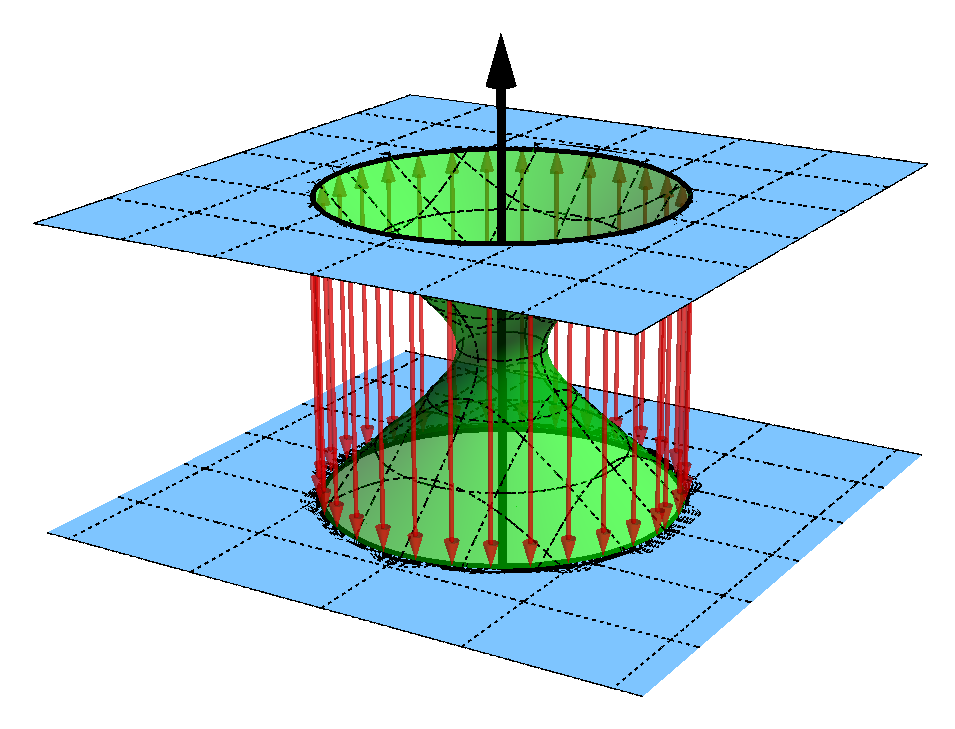
\includegraphics[width=.9\textwidth]{img/Chapter2/Identification.png}}
 \end{center}
 \caption{Pictoric image showing the identification process between the $x^2+y^2<a^2$ disks. The red arrows indicate that the two disk are glued together (not the rings) and there is no ``space'' between the two planes in this representation. The blue planes represent the $z=0$ planes in the $r>0$ and $r<0$ spaces. The green surface only serves to show the wormhole product of the identification but as the two disks are glued together, this surface does not exist in reality. Notice that in this representation the space between the two planes does not exist and therefore there is only displayed the $z>0$ semi-space of the upper copy of $\mathbb{R}^3$ and the $z<0$ semi-space of the lower copy of $\mathbb{R}^3$. The other semi-space are not in the picture as we would need another one to display them. We remark that as the green surface does not exist, topological properties cannot be derived from it. Moreover, the topology of the identification is trivial. }
 \label{fig:Identification}
\end{figure}  
It was first noticed by Brandon Carter \cite{carter1968global} that the Kerr spacetime can be extended beyond the previous description. This extension takes its origin in the fact that the Kerr metric in \gls{BL} coordinates is no singular at $r=0$ and therefore the variation range of this coordinate (initially $r\in(0,\infty)$) can be extended to $r\in(-\infty,\infty)$. This is due to the fact that the singularity is not a point but a ring. This identification is very easy to perform in \gls{KS} coordinates. First of all notice that if we restrict the values of the function $r=r(x,y,z)\in(0,\infty)$, then a geodesic that is defined along the $z$ axis ($x=y=0$) starting from the positive branch ($z>0$) will reach the disk inside the singular ring (located at $z=0,x^2+y^2<a^2$) with no problems because the inner disk is not singular, but there is still problems. For the $z>0$ axis the definition of the function $r$ that follows from \cref{eq:rdefinition} (with positive sign) is $r(x,y,z)=z$ and when the geodesic reaches the inner disk and passes through it, the definition of the function $r$ must change to $r(x,y,z)=-z$ as now $z<0$ and the function $r$ must remain positive. This change of sign in the function $r$ leads to a discontinuous definition as well as  to discontinuous curvature invariants  (like $R^{\alpha \beta \gamma \delta} R_{\alpha \beta \gamma \delta}$ (where $R^{\alpha}_{\beta \gamma \delta}$is the Riemann tensor). To remove this singularity we must extend the variation range of the function $r$ to $r(x,y,z)\in(-\infty,\infty)$ which leads to a identification between two copies of the Kerr spacetime.

\begin{proposition}
 The Kerr spacetime once the function $r(x,y,z)$ is extended to $r\in(-\infty,\infty)$ is foliated by the leafs 
 \begin{equation}
  \mathcal{M} = \frac{\mathbb{R}_+^3 \cup  \mathbb{R}_-^3}{\sim}
 \end{equation}
where in each leaf the time coordinate has a different value (which defines the foliation), $\mathcal{M}$ denotes the final \gls{MAE} manifold, $\mathbb{R}_+^3$ and $\mathbb{R}_-^3$ denotes two copies of $\mathbb{R}^3$ and $\sim$ is the equivalence relation given by
\begin{align}
 &p_1=(x_1,y_1,z_1) \in \mathbb{R}_+^3 \nonumber, \\
 &p_2=(x_2,y_2,z_2) \in \mathbb{R}_-^3 \nonumber, \\
 &p_1 \sim p_2 \longleftrightarrow \{ x_1=x_2, y_1=y_2 ,z_1=z_2=0, x_i^2+y_i^2<a^2 \}
\end{align}
The tangent planes are identified in the following way
\begin{align}
 &v_1 \in T_p\mathbb{R}_+^3,\quad \quad p \in x_1^2+y_1^2<a^2, z=0\\
 &v_2 \in T_p\mathbb{R}_-^3,\quad \quad p \in x_1^2+y_1^2<a^2, z=0\\
 &v_1 \sim v_2 \longleftrightarrow v_1^\alpha = v_2^\alpha.
\end{align}
The function $r(x,y,z)$ after de identification takes the form
\begin{align}
  r(x,y,z)&=\lambda \frac{\sqrt{\sqrt{\left(a^2-x^2-y^2-z^2\right)^2+4 a^2 z^2}-a^2+x^2+y^2+z^2}}{\sqrt{2}}\\
 \end{align}
 with $\lambda=1$ for $\mathbb{R}_+^3$ and $\lambda=-1$ for $\mathbb{R}_-^3$.
\end{proposition}
\begin{Proof}
 The implicit definition of the function $r$ in \gls{KS} coordinates given by \cref{eq:rdefinition} reads
 \begin{equation}\label{eq:rrelationident}
  r^2 \left(a^2+r^2\right)=z^2 \left(a^2+r^2\right)+r^2 \left(x^2+y^2\right).
 \end{equation}
 This equation have four solutions, two of them always real and the other two always imaginary (they are complex conjugate). The two real solutions are
 \begin{align}
  r(x,y,z)&=\frac{\sqrt{\sqrt{\left(a^2-x^2-y^2-z^2\right)^2+4 a^2 z^2}-a^2+x^2+y^2+z^2}}{\sqrt{2}}\\
  r(x,y,z)&=-\frac{\sqrt{\sqrt{\left(a^2-x^2-y^2-z^2\right)^2+4 a^2 z^2}-a^2+x^2+y^2+z^2}}{\sqrt{2}}
 \end{align}
  \begin{figure}   
\begin{center}
 \centerline{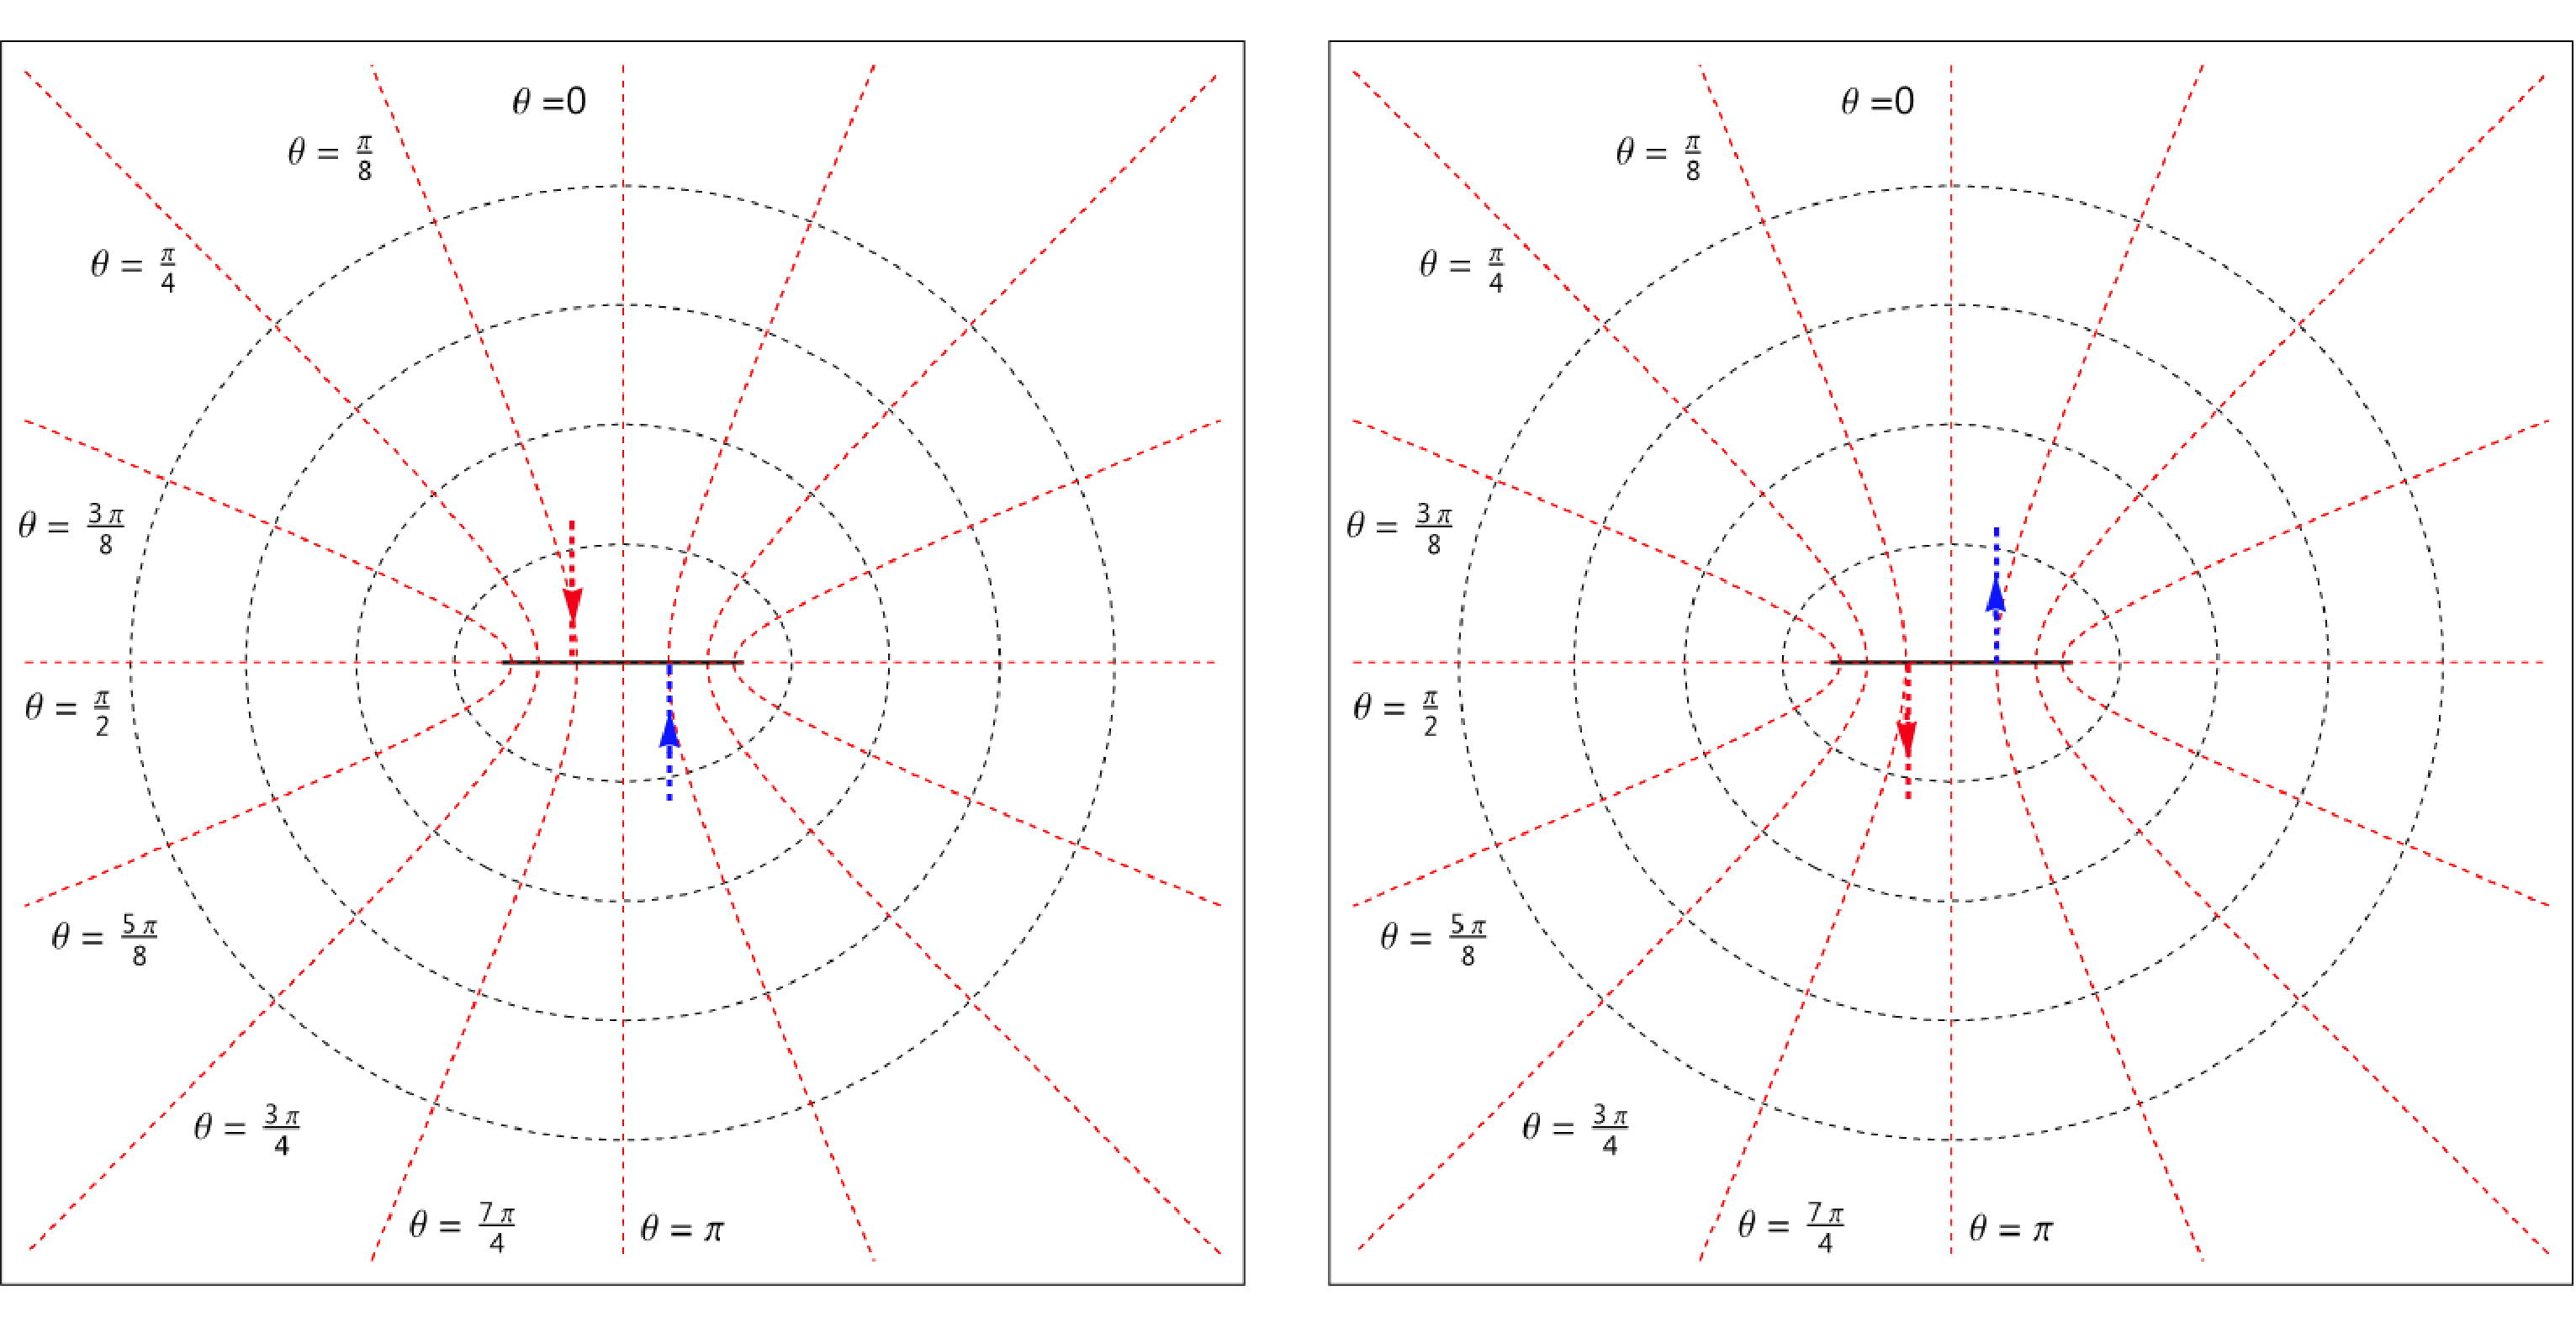
\includegraphics[width=\textwidth]{img/Chapter2/Idetification2.pdf}}
 \end{center}
 \caption{Side view of the spaces $\mathbb{R}_+^3$ (left image) and $\mathbb{R}_+^3$ (right image). The red dotted lines represent the surfaces with $\theta=const.$ while the black dotted lines represent the $r=const.$ surfaces.The singular ring is the thick black line in the middle. The arrows show how the identification works: A geodesic that follows the red arrow in the left image emerges in the right image following the red arrow and equivalently for the blue arrow. Once in the right image the situation becomes the same as it started. Note that a geodesic following one arrow can surround the ring and pass through the disk as the other arrow. As the green surface does not exist, the topological implications of its shape are inexistent, as the identification has trivial topology. }
 \label{fig:Identification2}
\end{figure} 
This is the reason that for each set of \gls{KS} coordinates there are two different values of $r(x,y,z)$. Therefore we have two different copies of the Kerr spacetime described by the metric \cref{eq:metricinKS} with different sign in the definition of the function $r(x,y,z)$. Let's name this copies $\mathbb{R}_+^3$ and $\mathbb{R}_-^3$. When we perform the similarity relation given by \begin{align}
 &p_1=(x_1,y_1,z_1) \in \mathbb{R}_+^3 \nonumber, \\
 &p_2=(x_2,y_2,z_2) \in \mathbb{R}_-^3 \nonumber, \\
 &p_1 \sim p_2 \longleftrightarrow \{ x_1=x_2, y_1=y_2 ,z_1=z_2=0, x_i^2+y_i^2<a^2 \}
\end{align}
we are constructing a topological manifold product of gluing the two disks together. In order to construct a differential manifold, we must say how we identify the tangent planes. They are under the following similarity relation:
\begin{align}
 &v_1 \in T_p\mathbb{R}_+^3,\quad \quad p \in x_1^2+y_1^2<a^2, z=0\\
 &v_2 \in T_p\mathbb{R}_-^3,\quad \quad p \in x_1^2+y_1^2<a^2, z=0\\
 &v_1 \sim v_2 \longleftrightarrow v_1^\alpha = v_2^\alpha.
\end{align}
Under this identification of the disks and the tangent planes, we are finally identifying the top the disk $x_1^2+y_1^2<a^2$,$z_1=0$ with the bottom of the disk $x_2^2+y_2^2<a^2$,$z_2=0$ and vice versa as is displayed in \vref{fig:Identification,fig:Identification2}. After the identification is complete, the definition of the function $r(x,y,z)$ becomes
\begin{align}\label{eq:rdefinitiondef}
  r(x,y,z)&=\lambda \frac{\sqrt{\sqrt{\left(a^2-x^2-y^2-z^2\right)^2+4 a^2 z^2}-a^2+x^2+y^2+z^2}}{\sqrt{2}}\\
 \end{align}
 with $\lambda=1$ for $\mathbb{R}_+^3$ and $\lambda=-1$ for $\mathbb{R}_-^3$. As the function r becomes $r(x,y,z)=0$ at the disk, we have a continuous and at least $C^2$ definition and therefore the curvature scalars are continuous. We must proof that this definition for the function $r(x,y,z)$ is also analytic. To achieve this, write for points near the inner disk ($x^2+y^2<a^2$ and $z\sim 0$)
 \begin{equation}
  r(x,y,z)=z \sqrt{f(x,y,z)}
 \end{equation}
where $f(x,y,z) : \mathbb{R}^3 \to \mathbb{R}^+$ is a everywhere positive function. Under this ansatz we can rewrite \cref{eq:rrelationident} as
\begin{equation}
 f(x,y,z) \left(z^2 f(x,y,z)+a^2-x^2-y^2-z^2\right)-a^2=0
\end{equation}
which leads to
\begin{equation}
  f(x,y,z)=\frac{\pm \sqrt{\left(-a^2+x^2+y^2+z^2\right)^2+4 a^2 z^2}-a^2+x^2+y^2+z^2}{2 z^2}
\end{equation}
to obtain a positive function we must chose the $+$ in the square root. This function satisfies that
\begin{equation}
 \lim_{z\to0}{f(x,y,z)}=\frac{-a^2}{-a^2+x^2+y^2}
\end{equation}
The function $f(x,y,z)$ is a analytic function because it is the result of composing analytic functions. As the function $z$ under the identification is continuous and analytic, we conclude that the function $r(x,y,z)$ is continuous because is the product of analytic functions. This is also because
\begin{equation}
 \lim_{z \to 0}{ z \sqrt{f(x,y,z)}}|_{x^2+y^2<a^2}=0
\end{equation}
As now the manifold is formed under a identification that leads to continuous and smooth functions and curvature scalars, we have removed the ``singularity'' across the disk. Of course, this corresponds only to the spatial part of the Kerr spacetime, i.e each foil of the whole foliation, where each foil has a different value of the time coordinate $t$.
\end{Proof} 

With this identification of the inner disk, a geodesic that falls through the $z>0$ branch of the $z$-axis with $r>0$ ($\mathbb{R}_+^3$ copy), reach the top of the inner disk at $x^2+y^2<a^2$,$z=0$ and emerges on the bottom of the inner disk of the space with $r<0$ ($\mathbb{R}_-^3$ copy). At this point, the geodesic can go to the asymptotically flat limit $r\to -\infty$. Is important to note that in the $\mathbb{R}_-^3$ copy, there are no horizons as the singularity equation $\Delta(r)=0$ only gives positive solutions for the horizons. 

As the geodesics are not necessarily defined on the $z$-axis, to fully understand this part of the Kerr \gls{MAE}, we must think in the spacetime as two complete and independent copies of $\mathbb{R}^3$. Imagine that in the two copies there is a disk inside the singular ring. If the identification is not yet done, if we travel across this disk nothing happens, i.e. if a geodesic goes from under the disk it will emerge above the disk and vice versa. This is obvious because we are only passing through a disk in a ``regular space''. Imagine now that after the identification is done, the behavior of the geodesic is the same (in the sense that if you pass through the disk from underneath you will emerge from the top and if you go across the disk from the top you will emerge from the bottom) but when you pass across the disk, you emerge in another space (another copy of $\mathbb{R}^3$) in the same way (top to bottom and bottom to top). Each copy is complete in the sense that have everything that the other copy have. Therefore, there are two different $z$-axis (one in each copy), two different singular rings (but only one disk because the identification is between the disks and no between the singular rings), two different asymptotically flat ends of the spacetime... The only thing that is not analogous between the two copies is that in $\mathbb{R}_-^3$ there is no horizons and the only singular surface is the singular ring, as was noticed previously.

Notice also that the \gls{MAE} of a geodesic that is imposed to move along the $z$-axis is formed by two disjoint parts. This is because if we consider a geodesic falling along the $z$-axis with $z>0$ in $\mathbb{R}_+$ when it reaches the inner disk, it emerges in $\mathbb{R}_-$ with $z<0$. As the geodesic is imposed to move along the axis, it cannot surround the ring and access the $z>0$ branch of $\mathbb{R}_-$ so this geodesic is forced to move in the space $\mathcal{Z}_1=\mathbb{R}_+|_{z>0} \cup \mathbb{R}_-|_{z<0}$. Similarly a geodesic that falls along the  $z$-axis with $z<0$ is forced to move in the space $\mathcal{Z}_2=\mathbb{R}_+|_{z<0} \cup \mathbb{R}_-|_{z>0}$. Indeed, the definition of the function $r(x,y,z)$ for a geodesic that falls along the $z$-axis ($x=y=0$) becomes
\begin{align}
 r(z,0,0)= \lambda z
\end{align}
with $\lambda=1$ for the space $\mathcal{Z}_1$ and $\lambda=-1$ for the space $\mathcal{Z}_2$.

 
\FloatBarrier
\section{Kerr-Schild patches}
  \begin{figure}[hpt!] 
\begin{center}
 \centerline{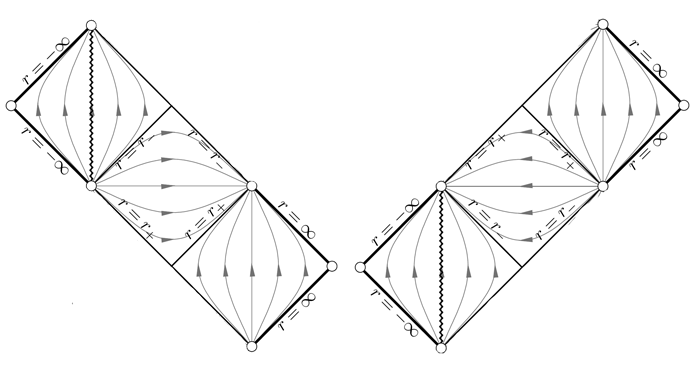
\includegraphics[width=.8\textwidth]{img/Chapter2/KerrSchild.png}}
 \end{center}
 \caption{The figure on the left shows the ingoing Kerr-Schild patch ($\sigma=-1$) while the figure on the right shows the outgoing Kerr-Schild patch ($\sigma=1$).}
 \label{fig:PenroseKS}
\end{figure} 
Actually the \gls{MAE} of the Kerr spacetime is much larger than the ring identification. We are going to study which part of the known maximal extension of the spacetime is covered by each \gls{KS} patch and how they are assembled. To do this we must know how the \gls{KS} time coordinate is related to the \gls{BL} time coordinate. From \vref{eq:Kerrcoordtrans1,eq:timeeq2} we can relate the \gls{KS} coordinate $t$ to the \gls{BL} analogue $\bar{t}$:
\begin{equation}
 d\bar{t}=dt+\sigma \left(\frac{r^2+a^2}{\Delta}-1\right).
\end{equation}
A direct integration for constant-$t$ trajectories gives
  \begin{equation}
 \bar{t}(r)=M \sigma  \left(\log \left(a^2-2 M r+r^2\right)+\frac{2 M \tan^{-1}\left(\frac{r-M}{\sqrt{(a-M) (a+M)}}\right)}{\sqrt{(a-M) (a+M)}}\right).
\end{equation}
The outer horizon is located at $r_+=M+\sqrt{\left(M^2-a^2\right)}$ and we can evaluate the function $\bar{t}(r)$ as it reaches the outer horizon, which gives that
\begin{align}
 \lim_{r \to r_+}{ \bar{t}(r)}|_{t=const.} &= - \sigma \infty,\\
 \lim_{r \to \infty}{ \bar{t}(r)}|_{t=const.} &=  \sigma \infty.
\end{align}
  \begin{figure}[htp!]
\begin{center}
 \centerline{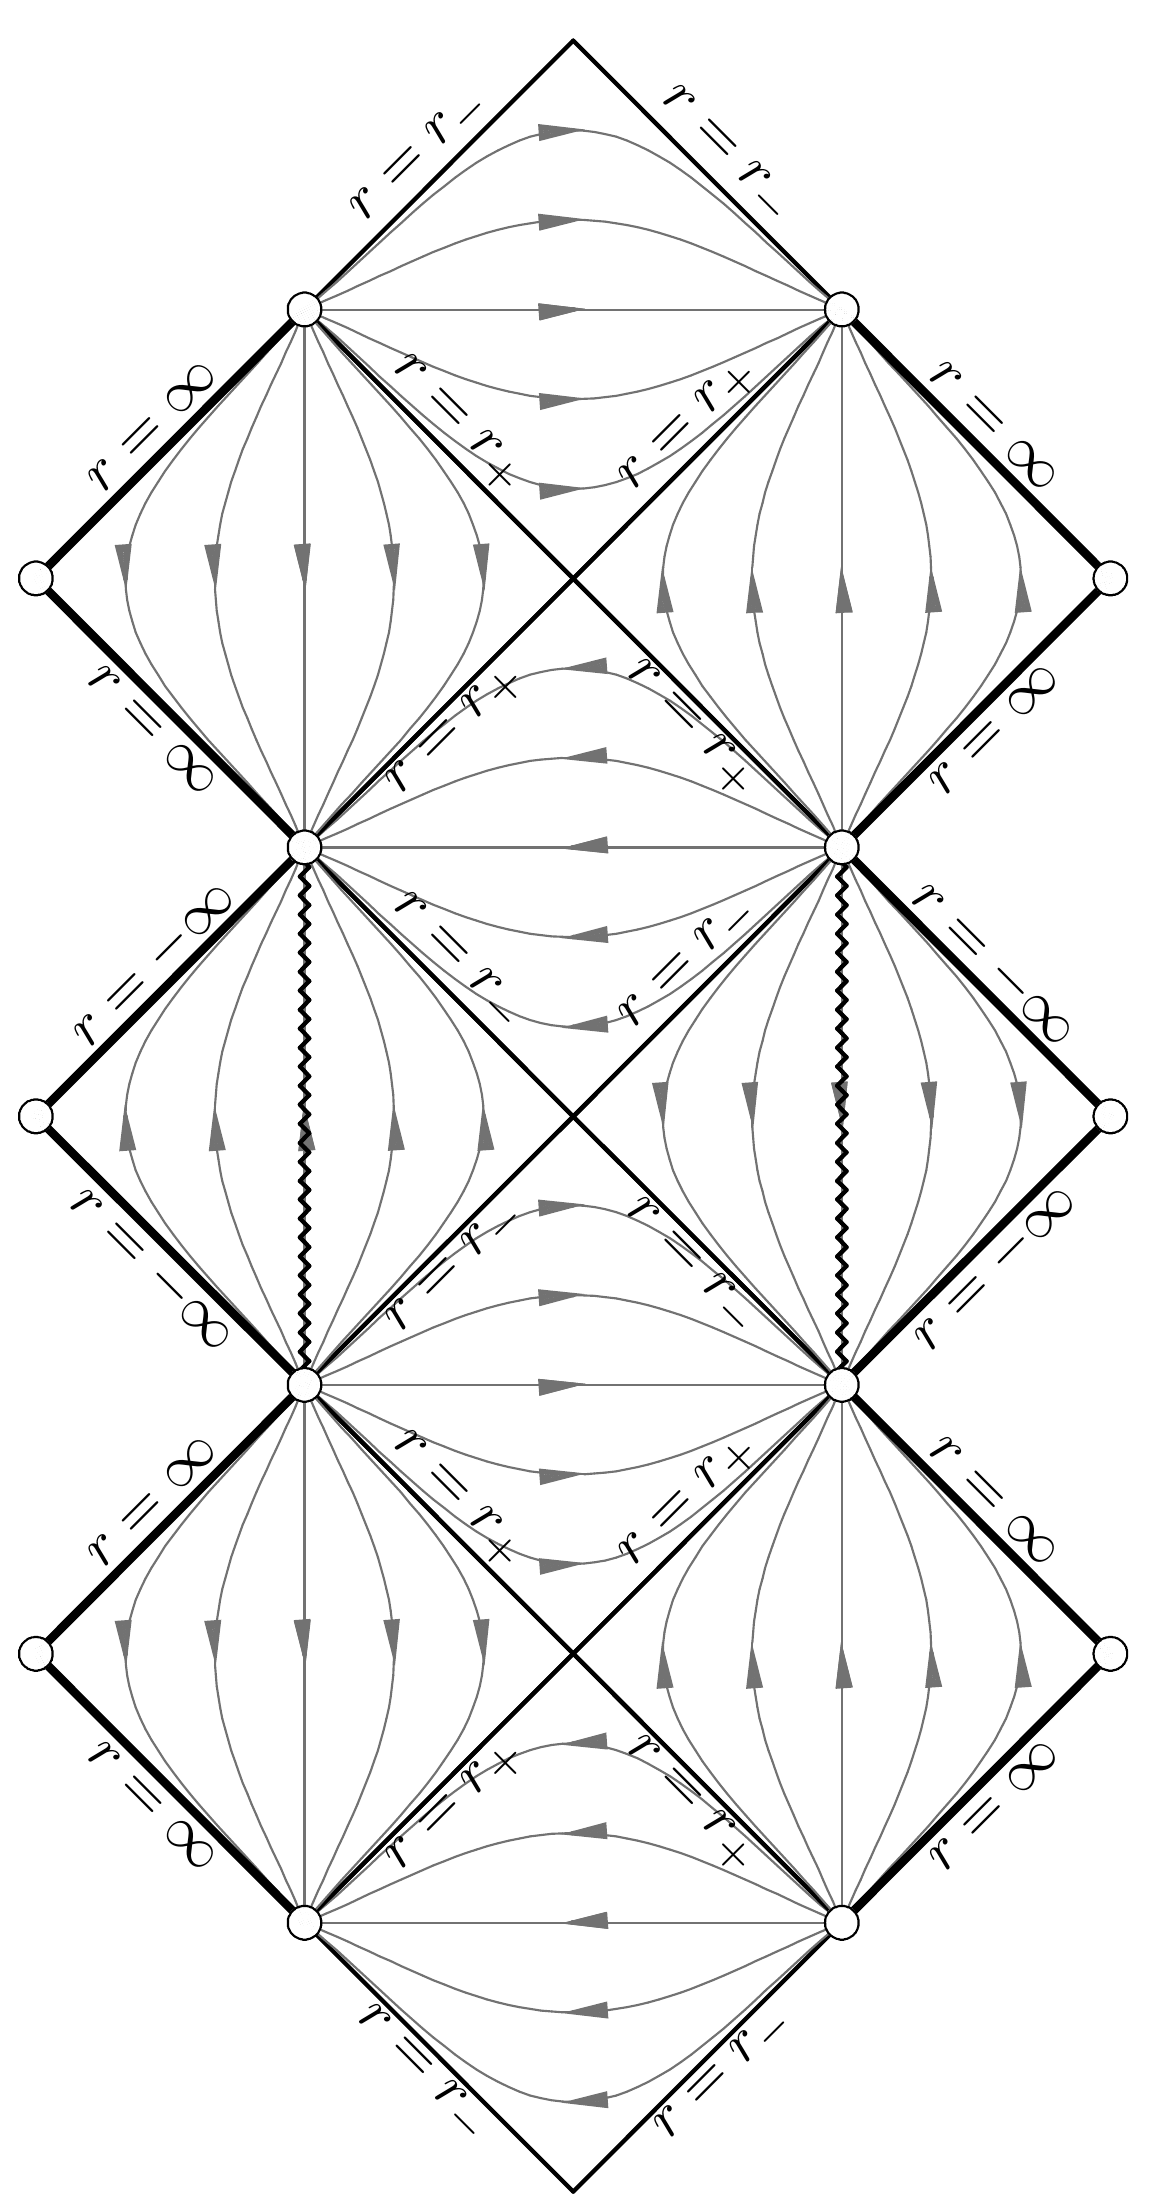
\includegraphics[width=.4\textwidth]{img/Chapter2/Diagrama.png}}
 \end{center}
 \caption{\gls{PC} diagram of the Kerr spacetime along the axis of symmetry for simplicity. The \gls{PC} diagrams are conformal compactifiactions of the spacetime that help to understand the causal structure of the whole manifold. The diagram is constructed to maintain the light cones as straight lines at $\frac{\pi}{2}$ \textit{rad}. For more information and resources to understand \gls{PC} diagrams see \cite{o1995geometry,hawking1973large}.}
 \label{fig:Penrose}
\end{figure} 
Therefore the Kerr-Schild patch with $\sigma=-1$ approaches $r \to r_+$ with $\bar{t} \to \infty$ and comes from $r=\infty$ in the past ( $\bar t=-\infty$ ) and the Kerr-Schild patch  with $\sigma=1$ approaches $r=\infty$ with $\bar{t} \to \infty$ and comes from $r \to r_+$  in the past ( $\bar t=-\infty$ ). We will assign (as is usually done in the \gls{SW} case) the denomination  \textit{Black hole} to the \gls{KS} patch with $\sigma=-1$ and \textit{White hole} to the \gls{KS} patch with $\sigma=1$. Of course, in \gls{KS} coordinates, the geodesic flow does not stop at $r_+$ and can be extended over $r_-$ until reaches $r=0$ for both values of $\sigma$. This two patches can be glued together an indefinitely number of times, allowing the geodesic flow to pass over $r_+$ and $r_-$ as many times as needed. A in-depth study of the geodesic completeness (see chapter 3 of \cite{o1995geometry}) reveal that the basic structure of the maximal extension is in reality formed by four basic patches (two of them isometric to the other two) as one can visualize in the Penrose carter diagram of \cref{fig:Penrose}. The two basic patches of the left are isometric to the two basic patches of the right (these two basic patches are the ones that we have studied), and this group is glued together and infinite number of times conforming the Penrose Carter diagram. The whole \gls{MAE} of the Kerr spacetime is not globally hyperbolic and also, if we can connect two points in the spacetime with a causal curve is not necessary true that there is a geodesic that connect this two points. Despite the \gls{MAE} is not globally hyperbolic, the two \gls{KS} patches are globally hyperbolic and therefore it is true that if we find a causal curve connecting two points, exists a geodesic that connect the same points. This is quite useful to think in the different geodesic trajectories that we are going to describe in the next chapters. As a geodesic can be extended across the \gls{PC} diagram, it can travel infinitely across the \gls{KS} regions and escape to one of the asymptotically flat regions in $r=\infty$, end in the ring singularity or even pass through one of the inner disks (one of the infinite disk in the middle of the singular rings) and cross to one of the $\mathbb{R}_-^3$ copy of the spacetime. As we can see, the geodesic behavior in the whole spacetime is very complicated even if we restrict the movement to the $z$-axis. But as we will see in the next chapters, we are going to develop a method that allows us to describe all the complicate geodesic trajectories in one simple and 2D phase space where all possible geodesics will be displayed. 

\section{Causality violations}
\begin{figure}
\begin{center}
 \centerline{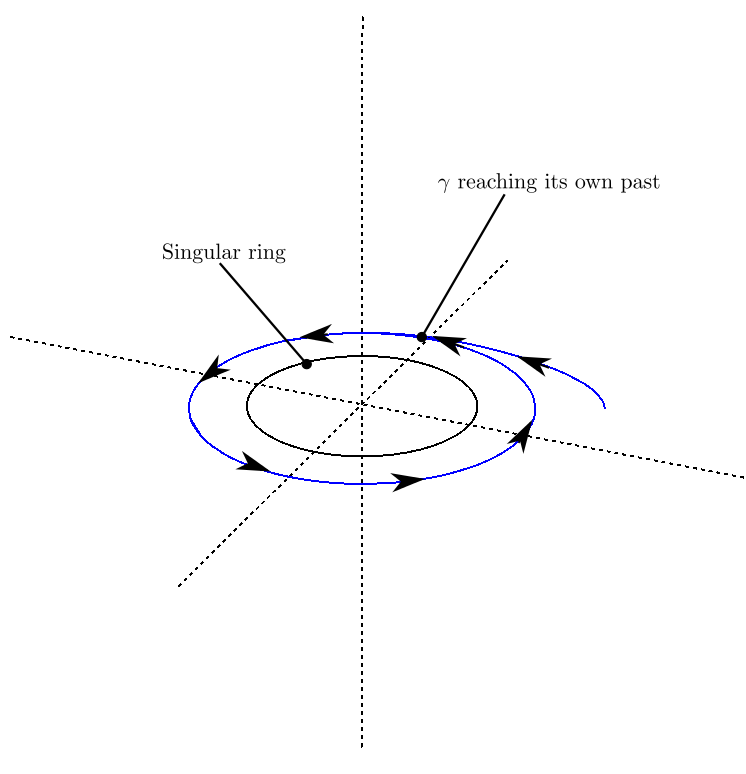
\includegraphics[width=.75\textwidth]{img/Chapter2/causal.png}}
 \end{center}
 \vspace{-1cm}
 \caption{The curve $\gamma$ as it reaches its own past.}
 \label{fig:pastgamm}
\end{figure} 
We have seen that in the region $\mathbb{R}_{-}^3$ the value of the coordinate $r$ is bounded in the interval $[-\infty,0]$. We are going to see that this lead to causality violations. This causality violations are closed causal curves that can correspond to physical observers (timelike curves with $u^\alpha u_\alpha<0$, where $u^\alpha$ is the tangent vector), which lead to time travel as the curve reach his own past for finite value of the propper time. This is easier to show in \gls{BL} coordinates. Let us consider a timelike curve $\gamma$ consisting a circle in the equatorial plane outside the singular ring in the space $\mathbb{R}_{-}^3$. This curve is defined as
\begin{equation}
 \gamma \equiv \quad \{ \bar{t}=const. \quad \theta=\frac{\pi}{2} \quad 0 \leq \bar{\phi} \leq 2 \pi \quad r<0\}.
\end{equation}
This curve can be the curve of an observer which stats in $\mathbb{R}_{+}^3$, crosses the two horizons, pass through the inner disk and goes around the equatorial plane just outside the singular ring. The norm of the tangent vector is
\begin{equation}
\begin{aligned}
  u^\alpha u_\alpha&=\frac{1}{r^2} \left((r^2+a^2)^2 - a^2 (r^2+a^2-2M r) \right) \nonumber \\
  &=\frac{1}{r^2}(r^4+r^2 a^2+2 M r a^2)=r^2+a^2+\frac{2 M a^2}{r}
  \end{aligned}
\end{equation}
If we set $|r|<<a,M$ (which we can do because the ring singularity is at $r=0$) we will have that $r^2+a^2+\frac{2 M a^2}{r}<0$ and the curve is a timelike curve that correspond to a physical observer. As the curve is a closed curve because is a ring, the curve reach itself in its own past. In any case, this is not a physical problem, as the space  $\mathbb{R}_{-}^3$ is beyond the even horizon and then cannot be observed (at least as long as we do not fall inside the black hole).

